\chapter{Within-Day Replanning}
\label{ch:withinday}
% ##################################################################################################################

\hfill \textbf{Authors:} Christoph Dobler, Michal Maciejewski, Kai Nagel

\begin{center} 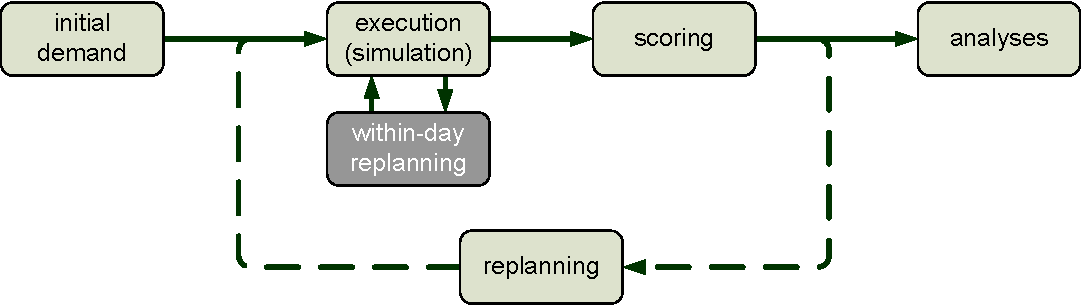
\includegraphics[width=0.6\textwidth, angle=0]{extending/figures/WithinDayReplanning/WithinDayMATSimLoop} \end{center}

% ##################################################################################################################
\section{Introduction}
In recent years, in transport planning and traffic management the interest in scenarios where events occur which cannot or only partially be foreseen has increased. Typical examples for events which can only partially be foreseen are taxis and car sharing. An agent that has a taxi trip in its plan can for example not know in advance which taxi will be available when the agent needs one. When using car sharing, an agent might walk to the car sharing station and check whether a car is available or not. In case it is not, the agent could either decide to wait or adapt its plan and switch to another mode. Examples for events which cannot be foreseen at all are road accidents, terrorist attacks or disaster such as earthquakes.

Traditional simulation approaches (as used in MATSim) optimize traffic demand using an iterative process. There, it is assumed that a typical situation is simulated where agents can rely on their experience from comparable situations, like previous iterations. Applying an iterative approach to a scenario with unexpected events results in problems like illogical agent behaviour, producing false results. In the next section, these problems, as well as an alternative simulation approach, are presented. On one hand, this approach---called within-day replanning---simulates only a single iteration, avoiding problems resulting from an iterative simulation process. On the other hand, this approach does require a more detailed behavioral model for the agents. Subsequently, using MATSim as a base, the iterative approach is discussed, followed by two different implementations of the within-day replanning approach into the framework including discussions of the technical implementations.


% ##################################################################################################################
\section{Simulation Approaches} \label{sec:SimulationApproaches}
\subsection{Iterative Simulation Approaches} \label{sec:IterativeSimulationApproaches}
% ============================================================================================
The starting point of an iterative simulation approach, as it is used in agent-based traffic flow micro-simulations like DYNEMO \citep{Schwerdtfeger_VolmulerHamerslag_1984, NoekelSchmidt_NSE_2002}, MATSim \citep{Balmer_PhDThesis_2007, BalmerEtAl_HEUREKA_2008} or TRANSIMS \citep{SmithEtAl_NTRPAC_1995, NagelRickert_ParComp_2001},  is the generation of an initial plan for each agent (e.g.\ based on census and~/~or travel diary data). A plan contains an agent's intended schedule of activities and the trips that connect them. For each activity, its type (e.g.\ \emph{work}, \emph{leisure} or \emph{shopping}), its location and the expected start and end time are given. A transport mode and a route specify a trip. The iterative optimization process consists of three steps. First, a mobility simulation executes the plans which are then evaluated using a fitness function. Finally, agents must select plans to be executed in the next iteration. Each agent can keep several plans in its memory. Bad plans can be deleted and new plans created by cloning and adapting existing ones using information (e.g.\ travel times) from one or more previous iterations. The allowed adaption operations define the optimization search space (e.g.\ routes, location and start / end times of activities). This iterative optimization can be seen as a period-to-period replanning strategy. Since one day is a commonly used duration, it is often called day-to-day replanning strategy.

An iterative day-to-day replanning approach is appropriate as long as the scenario describes a typical situation or day. For such scenarios, it is feasible to assume that agents are familiar with typically occurring events like traffic jams during peak hours. Therefore, they try to avoid driving during those times, or use alternative routes with less traffic. However, if the scenario contains unexpected events that the agents cannot foresee (e.g.\ accidents or heavy weather conditions), using an iterative approach is not the best choice. First, user equilibrium will not be reached in such a scenario because agents do not have enough information to choose optimal routes and daily activity plans. Another problem is the optimization process itself. Even if an agent chooses its routes randomly due to a lack of information, it will eventually find a good route if it tries enough different routes.

%---------------------------------------------------------------------
\createfigure%
{Exceptional event in a network}%
{Exceptional event in a network}%
{\label{fig:labelExceptionalEventExample}}%
{%
  \createsubfigure%
  {Network with planned route}%
  {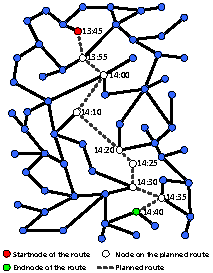
\includegraphics[width=0.43\textwidth, angle=0]{extending/figures/WithinDayReplanning/network_original_route}}%
  {\label{fig:labelNetworkPlannedRoute}}%
  {\qquad}%
  \createsubfigure%
  {Network with exceptional event}%
  {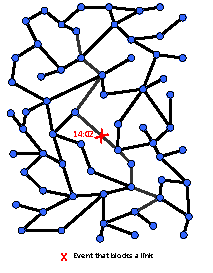
\includegraphics[width=0.43\textwidth, angle=0]{extending/figures/WithinDayReplanning/network_exceptional_event}}%
  {\label{fig:labelNetworkExceptionalEvent}}%
  {\vspace{5mm}}%

  \createsubfigure%
  {Network with exceptional event and planned route}%
  {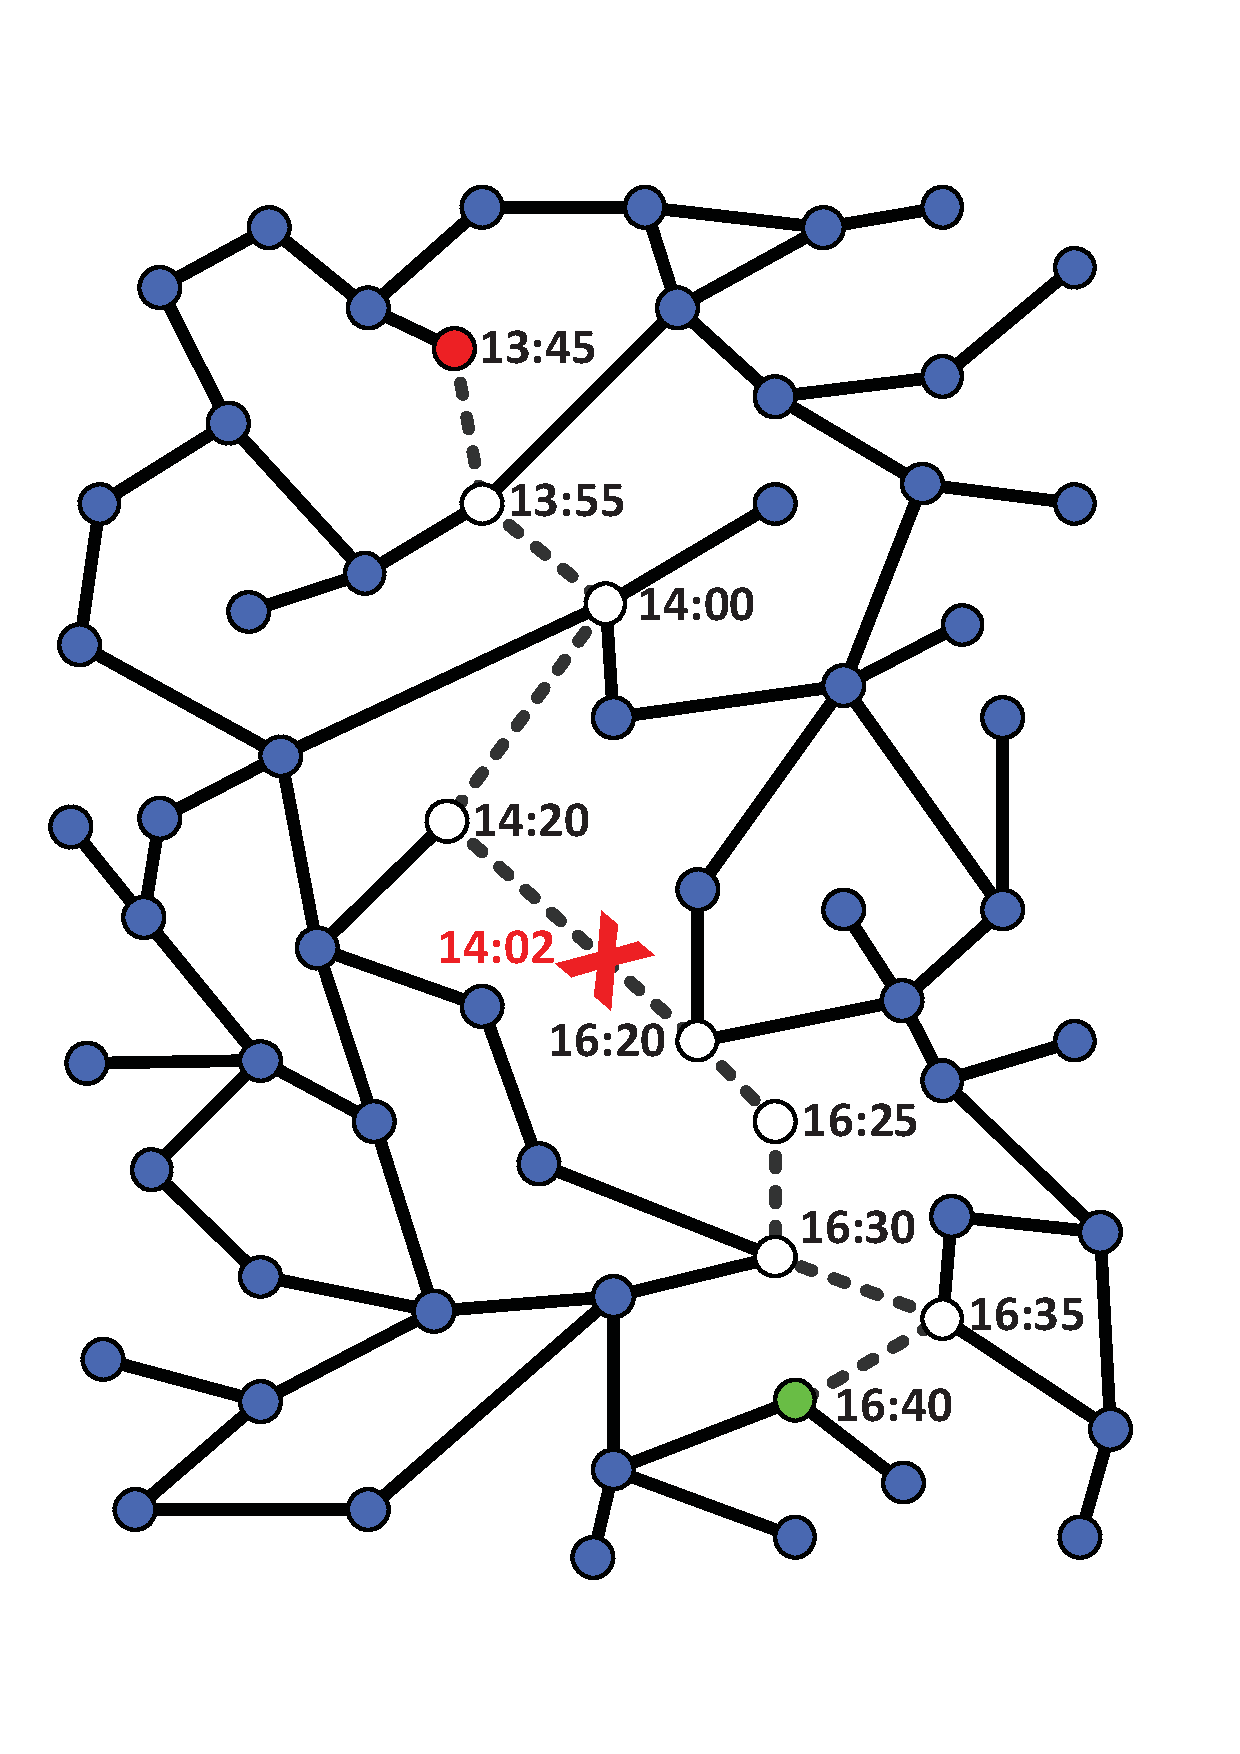
\includegraphics[width=0.43\textwidth, angle=0]{extending/figures/WithinDayReplanning/network_original_route_with_event}}%
  {\label{fig:labelNetworkExceptionalEventPlannedRoute}}%
  {\qquad}%
  \createsubfigure%
  {Network with exceptional event and adapted route}%
  {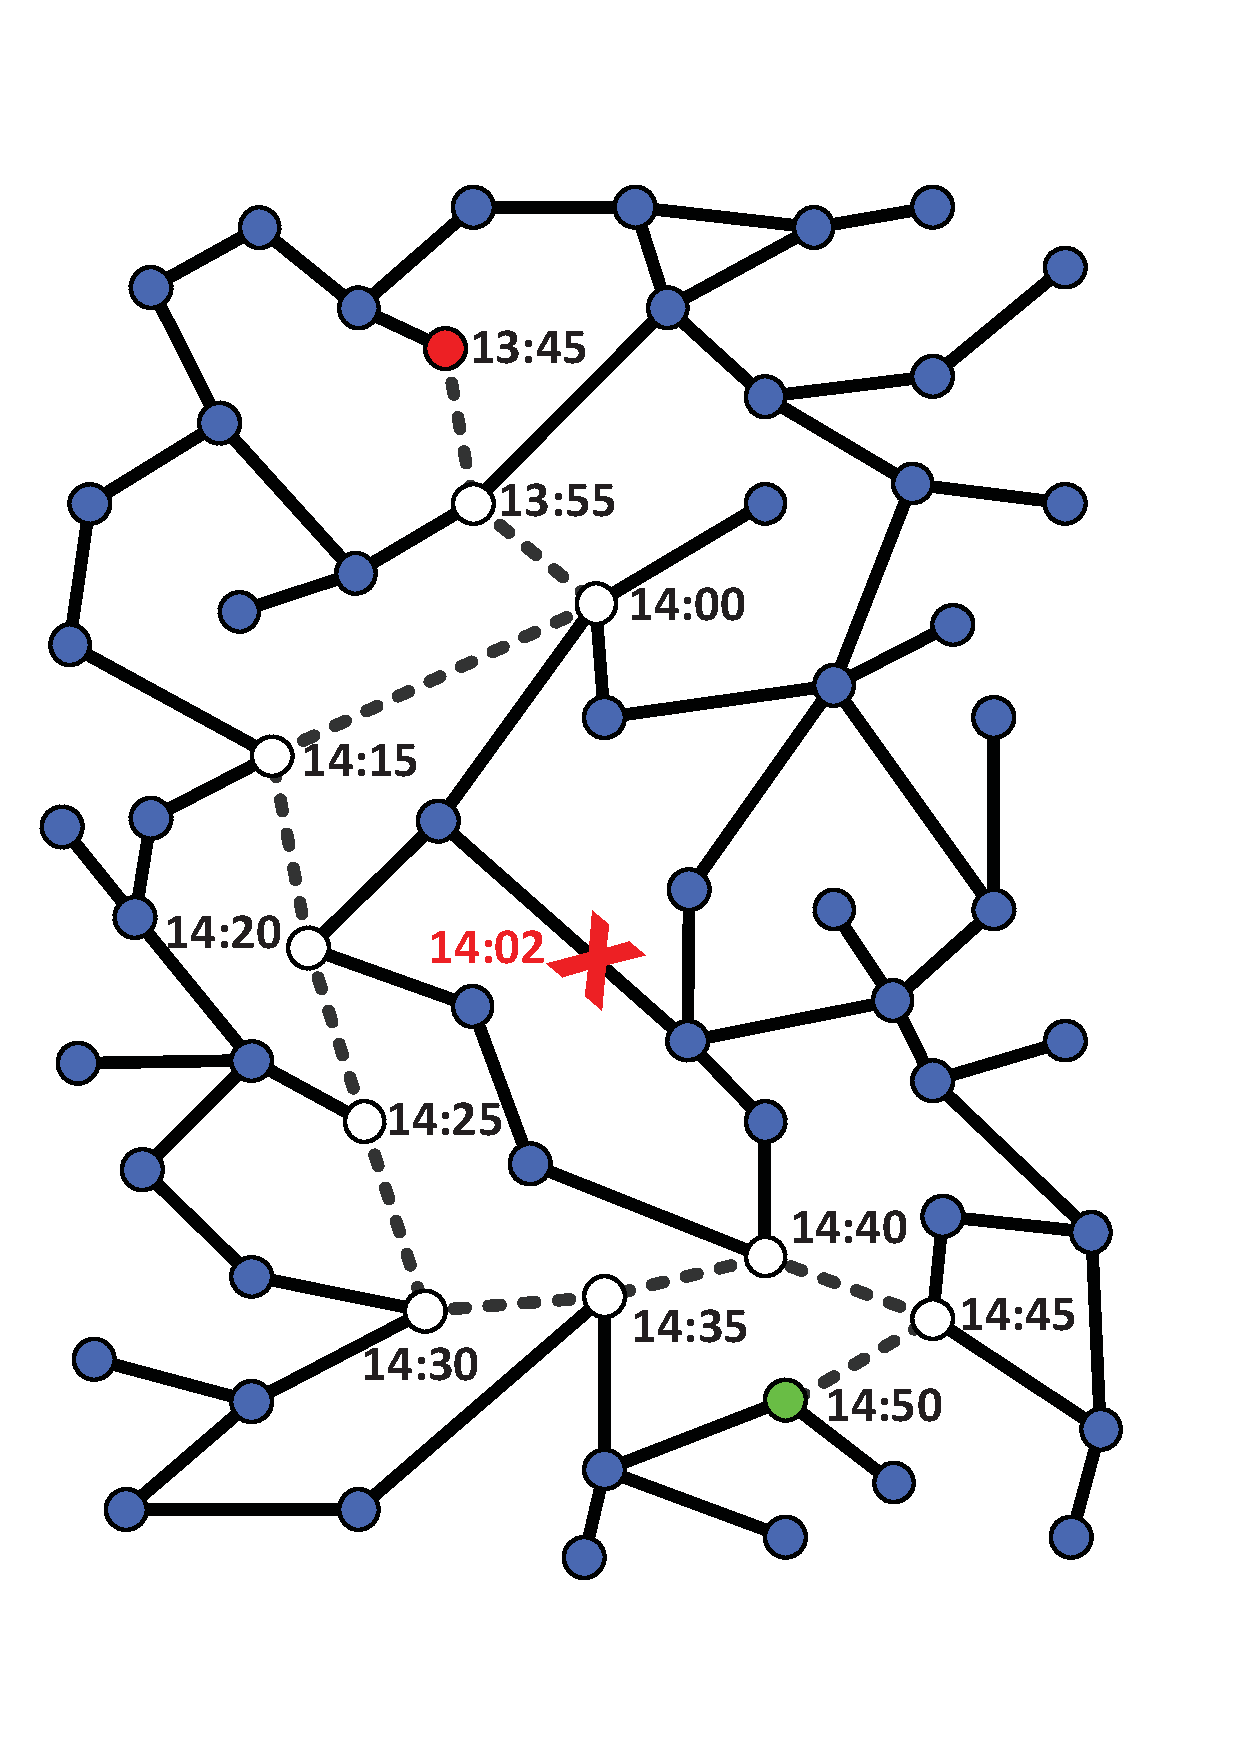
\includegraphics[width=0.43\textwidth, angle=0]{extending/figures/WithinDayReplanning/network_adapted_route_with_event}}%
  {\label{fig:labelNetworkExceptionalEventAdaptedRoute}}%
  {}%
}%
{}
%---------------------------------------------------------------------

Figure \ref{fig:labelExceptionalEventExample} shows a simple example scenario where an iterative approach would produce illogical and faulty results. In Figure \ref{fig:labelNetworkPlannedRoute} an agent's planned route in a sample network is shown, including the times when the driver passes each node of the route. Clearly, those times are only valid if no exceptional event occurs. Figure \ref{fig:labelNetworkExceptionalEvent} shows a link where an event, like an accident, blocks that link for two hours. As a result, the agent reaches its destination two hours later than expected (Figure \ref{fig:labelNetworkExceptionalEventPlannedRoute}). When this scenario is iterated, the agent recognizes that its route has a much higher travel time than expected and therefore it will choose another route. The traffic jam caused by the accident will probably also increase travel times on links next to the blocked link. Therefore, the agent might find a route which is quite different than the original one (Figure \ref{fig:labelNetworkExceptionalEventAdaptedRoute}). A closer look at the node where the new route deviates for the first time from the original one shows that this occurs even before the accident happened, which is unfeasible and illogical.

An obvious solution to avoiding such problems is using an alternative simulation approach without an iterative optimization process. The next section discusses such an approach and the requirements that must be fulfilled.

% ============================================================================================
\subsection{Within-Day Replanning Approach}
A within-day replanning approach uses a significantly different strategy from that of an iterative approach. Instead of multiple iterations, only a single one is simulated. Thus, it is now essential that agents can adapt their plans during this iteration without having information from previous iterations available. To do so, they have to continuously collect information and take into account their desires, beliefs and intentions when they decide how to (re)act.

While iterative approaches can use best-response modules, a within-day approach has to use something that might be called a best-guess module. Travel times are an obvious example. In an iterative approach, travel times can be collected from the previous iteration or even be averaged over several past iterations. The nearer a stable system is to a relaxed state, the smaller the differences in travel times between two iterations. This is not possible in a within-day approach. Even if an agent has perfect knowledge, it can only assume how the traffic flows will evolve in the future. To do so, it can take different information into account to estimate travel times. It could, for example, take travel times from a typical day without exceptional events and combine them with information it gathers during the simulated day. Depending on the amount and the quality of this information, the agent might rely more or less on its experience.

Therefore, the decision-making process of an agent becomes an important topic. In an iterative approach, each agent has total information and can thus select the best route. Due to limited available information, this is not possible in a within-day approach. One agent could, for example, choose a route where expected travel time is very short, but also very uncertain. Another agent might not be willing to take that risk and therefore select a longer route where the assumed travel time is more reliable. Perception of information might also vary between agents; one could rely on media traffic information, another might ignore it.

Each within-day replanning action is categorized by two parameters---the replanned element of the plan (an activity or a trip) and the point in time when the replanned plan element is executed (right now or at a future point in time). If an activity is replanned, several changes are possible. Its start and end time can be adapted, its location can be changed, it can be dropped, or created new from scratch. For a trip, origin and destination, route, mode of transport and departure time can be replanned. Often replanning one single plan element results in a chain reaction that forces replanning of other plan elements. If, for example, an activity is dropped, the trips from and to this activity have to be merged.

The second parameter categorizing a replanning action depends on when the replanned plan element is executed. This could be either the currently performed plan element or one being performed in the future. Clearly, in a currently performed plan element, not all previously mentioned replanning actions could be conducted. E.g.\ start time of an activity or transport mode of a trip currently being performed can no longer be adapted.

Due to the limited available information, a within-day replanning approach will, in contrast to an iterative approach, not converge to a user equilibrium. Decisions made during the simulated time period may seem to be optimal when they are made. However, evaluated retrospectively, an agent might realize that they were not.

Figure \ref{fig:labelWithinDayMATSimLoop} shows how within-day replanning can be integrated into MATSim's iterative optimization loop. An additional block builds another (inner) loop with the mobility simulation. Depending on the type of simulated scenario, the outer loop can be skipped.
%---------------------------------------------------------------------
\createfigure%
{(Iterative) within-day replanning MATSim loop}%
{(Iterative) within-day replanning MATSim loop \kai{I think this figure needs to come earlier, i.e.\ in Sec.~\ref{sec:SimulationApproaches} \textbf{TODO: redraw this figure using the new (blue) matsim loop?}.}}%
{\label{fig:labelWithinDayMATSimLoop}}%
{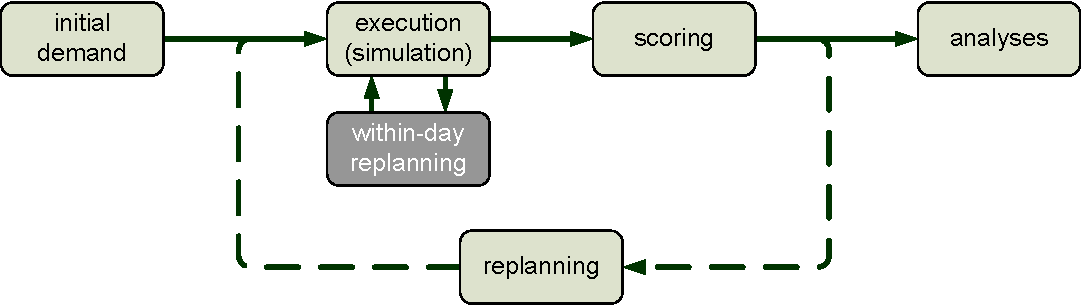
\includegraphics[width=12.5cm, angle=0]{extending/figures/WithinDayReplanning/WithinDayMATSimLoop}}%
{}%
%---------------------------------------------------------------------

% ============================================================================================
\subsection{Combined Approaches} \label{sec:CombinedApproaches}
An alternative to iterative or within-day replanning only approaches, is to combine them. An obvious application is solving situations that cannot be planned exactly in advance, like parking or car sharing. An agent is, for example, able to plan a parking activity, but it cannot anticipate which parking spots will be available when the agent arrives. Thus, within-day replanning can be used when the agent starts its parking choice.

Other agents might want to share their cars, so an actual meeting must be confirmed. This can be ensured using within-day replanning. If the driver arrives too early, a \emph{waiting} activity is added to its plan; otherwise the agent being picked up will perform a \emph{waiting} activity until the car arrives.


% ##################################################################################################################
\section{Implementation}
\subsection{General Thoughts}

Within-day or en-route replanning means that travelers replan during the day or while they are on their route.  This means that the simulation needs to find some way to influence the agent while the mobility simulation (network loading) is running.  For the \acrshort{matsim} main network loading module, the so-called \lstinline$QSim$, this could be achieved by inserting an agent-loop, as follows:
\begin{lstlisting}
   void doSimStep() {
      for ( each agent ) {   // <-- agent loop
         agent.doSimStep() ;
      }
      for ( each link ) {
         link.doSimStep() ;
      }
      for ( each node ) {
         node.doSimStep() ;
      }
   }  
\end{lstlisting}
In this loop, each agent has the chance to deliberate in every time step.  Clearly, the agent can decide that he/she has nothing to deliberate and return immediately.

Such an approach does, however, lead to computational challenges.  Going through all links and nodes in every time step is already an expensive operation, and a number of efficiency improvements (such as ``switching off non-active links'') are contained in the code.  Also, the number of links or nodes is typically an order of magnitude smaller than the number of synthetic persons in a scenario.  Thus, some massive optimization would have to be undertaken in order to make the above approach computationally efficient.

An alternative approach to the above is to ask each agent only when a decision needs to be taken.  The most important decision for a driver is to chose the next link, i.e.
\begin{lstlisting}
class MyDriverAgent implements DriverAgent {
   ...
   @Override
   public Id<Link> chooseNextLink() {
      <algorithm to determine ID of next link>
      return nextLinkId ;
   }
}
\end{lstlisting}
Similar implementations are needed for all other queries that could be asked of the agent, for example
\begin{compactitem}

\item Should the trip end on the current link?

\item Should the agent alight at the current stop?

\item What is the ID of the vehicle to be used for a trip?

\end{compactitem}
From the perspective of the agent such an approach might be called \emph{event driven}, since the agent performs mental activity only at such events.

There is, indeed, a mechanism to program such agents and to insert
them into the \lstinline$QSim$.  This is discussed in more detail in
Section~\ref{sec:impl-repl-the-ag}.

A challenge with that approach is that the complete agent needs to be re-programmed.  This agent needs to have enough capabilities to be oriented about itself; for example, it needs to be able to compute plausible routes.

On the other hand, there are situations where the capability to decide the turn at each intersection while en-route is, in fact, not needed.  
%
For example, for typical evacuation applications it makes sense to start all agents on their normal daily plans.  When an emergency warning is distributed, the simulation can go once through all agents and decide how they react.  This will be done by replacing some or all future elements of the current plan.  In some applications this may happen more than once, for example if the recommended evacuation directions change because of a change in wind direction.  In other applications, evacuating agents may become stuck in unexpected congestion which may trigger en-route re-routing.  This may, however, be restricted to relatively small regions, and it may be sufficient to go through such a replanning loop every, say, 300 simulated seconds. 

For such applications, the plan-based approach (Section~\ref{sec:impl-plan-based}) is more suitable.  Rather than having each agent answering certain queries in every time step or at every intersection, the plan-based approach first waits for a trigger (such as an emergency warning, or unexpected congestion), then decides on the affected agents, and then goes through those agents and changes the future portion of their plans.   This is not only conceptually easier than having every agent to answer for him-/herself, but it is also computationally more efficient since it is only called when it is triggered, and for the affected agents. 

Overall, implementers and users will have to balance their needs.  
%
If there are relatively few times when agents should re-plan, and these times can be easily identified by, say, corresponding to an emergency signal, then this is an indicator for the plan-based approach.  
%
If, on the other hand, an agent goes into the simulation mostly or entirely without a plan, for example for an entirely reactive taxi driver, then this points to the approach of replacing the agent.

\acrshort{matsim} provides infrastructure for both approaches.  The plan-based approach currently provides more support infrastructure, i.e.\ many important use cases can be implemented by re-using existing methods.  The approach that replaces the agent, in contrast, provides more flexibility.  In particular, it makes it possible without additional computational overhead that agents make decisions at the latest possible time.  While this is not entirely realistic behaviorally, such an approach is often desirable from a simulation perspective, where one does not want reproducibility of simulations depend on, say, random elements in terms of how far an agent plans ahead.



%%%%%%%%%%%%%%%%%%%%%%%%%%%%%%%%%%%%%%%%%%%%%%%%%%%%%%%%%%%%%%%%%%%%%%
\subsection{Implementation Alternative 1: Plan-Based Implementation}
\label{sec:impl-plan-based}
%%%%%%%%%%%%%%%%%%%%%%%%%%%%%%%%%%%%%%%%%%%%%%%%%%%%%%%%%%%%%%%%%%%%%%

\kai{Christoph, die ``mnote'' sind für mich, damit ich einen schnellen Überblick habe, was Du geschrieben hast.  Damit ich das nicht wiederhole, sondern mich ggf.\ darauf beziehe.}

\mnote{day-to-day loop no longer necessary}

When adding within-day replanning to MATSim, its iterative loop (see Figure \ref{fig:matsimcycle}) has to be adapted as shown in Figure \ref{fig:labelWithinDayMATSimLoop}. On one hand, the additional \emph{within-day replanning} module is added, which interacts with the mobility simulation. On the other hand, multiple iterations are only necessary if a combined simulation approach is used.

\mnote{implementation as MobsimEngine ... tracking agents and plans}

The implementation is realized as so-called \emph{MobsimEngine} which can be plugged into the \emph{QSim}. In every simulated time step, the \emph{QSim} iterates over all registered \emph{MobsimEngines} and allows them to simulate the current time step. Besides simulation of the traffic flows, those engines are also able to let agents start or end activities. The engine containing the within-day replanning logic (called \emph{WithinDayEngine}) does not simulate traffic flows but tracks agents and adapts their plans. Doing so is separated into two steps. First, agents whose plans have to be adapted in the current time step are identified. In a second step, the adaption of their plans is performed. 

\mnote{register identifiers with replanners, replanners with the within-day engine}

Figure \ref{fig:labelWithinDayEngine} shows the structure of the \emph{WithinDayEngine}. Multiple \emph{Replanners} can be registered to the engine. Each \emph{Replanner} represents a unique replanning strategy like re-routing or time mutation and uses a set of \emph{Identifiers} which communicate with agents and select those agents who are given the opportunity to adapt their plans. An \emph{Identifier} can be seen as an information-distributing unit, like a radio station or a policeman. Therefore, not every \emph{Identifier} communicates with all agents. For example, agents at home will probably listen to the radio, but agents walking in the park will not. Each \emph{Identifier} returns a list of agents to its superior \emph{Replanner}, which then adapts those agents' plans.

%---------------------------------------------------------------------
\createfigure%
{WithinDayEngine}%
{WithinDayEngine}%
{\label{fig:labelWithinDayEngine}}%
{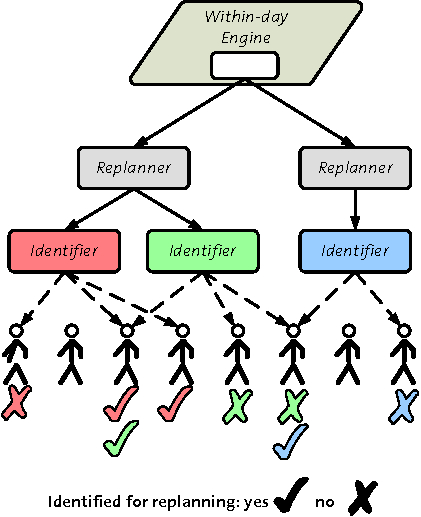
\includegraphics[width=8.0cm, angle=0]{extending/figures/WithinDayReplanning/ReplanningManager}}%
{}
%---------------------------------------------------------------------

\mnote{more about itentifiers and replanners}

There is a division of responsibilities between \emph{Replanners} and \emph{Identifiers}. The first ones are responsible for adapting the agents' plans but they should not check whether an agent should be replanned or not. If, for example, a \emph{Replanner} updates an agent's route, it has to be ensured by the \emph{Identifiers} that only agents who are currently performing a leg are replanned. In turn, \emph{Identifiers} should select agents who have to be replanned but should not change their plans. As a result of this division, the often time consuming replanning of the agents' plans can be performed using parallel threads which leads to an almost linear speed-up. In general, simulation results do not depend on the order in which agents are replanned. \emph{Replanners} which use random numbers are a special case. 
%They have to ensure that 
In the present implementation, their \emph{random number generator} is re-initialized for every replanned agent using a deterministic value (e.g.~a combination of the agent's Id and the current time step). On one hand, this ensures that an agent's decisions can be reproduced even when the global sequence of random numbers changes. On the other hand, the simulation outcomes do not change if the number of threads used for the replanning is changed.
% \kai{Christoph, ist es das?  ``have to'' (wie Du es vorher hattest), erscheint mir auf jeden Fall zu stark.  Oder hat es etwas mit multi-threading zu tun?}

\mnote{identifiers run sequentially}

Running the \emph{Identifier(s)} to select those agents who have to adapt their plans is performed sequentially. On one hand, an \emph{Identifier's} runtime is typically very short and therefore no significant performance losses are expected. On the other hand, 
%it is a robust design which 
this makes the design robust so it cannot produce race conditions which could occur if multiple instances of an \emph{Identifier} run concurrently. An example would be an \emph{Identifier} which selects agents on household level, i.e.~if a member of a household is identified, also all other members are added to the list of agents who have to be replanned. In an approach with parallel running instances of an \emph{Identifier}, an instance could identify member A of  a household while concurrently another instance could identify member B of the same household. As a result, the household's members would be twice in the list of agents to be replanned---once added by each \emph{Identifier} instance.

\mnote{different basic replanners for current/future trips/acts}

\emph{Replanner} implementations are available for every possible basic change of an agent's scheduled daily plan. Any trips and activities can be adapted, although some replanning operations are not available when trip or activity has already been started. Possible adaptations are:
\begin{compactitem}
    \item current trip (route, destination)
    \item future trip (add, remove, mode, route, origin, destination)
    \item current activity (end time)
    \item future activity (add, remove, location, type, start and end time)
\end{compactitem}
%
For complex plan adaptations, those basic \emph{Replanners} can be combined. If, for example, an agent currently performing a trip changes the destination of its next activity, routes of the current and next trip have to be adapted.

\mnote{different basic identifiers}

Additionally, four basic \emph{Identifiers} have been implemented so far. They identify agents, which are...
\begin{compactitem}
    \item performing an activity.
    \item performing an activity which will end in the current time step.
    \item performing a trip.
    \item performing a trip and are going to move to another link.
\end{compactitem}

\mnote{AgentFilters (e.g.\ for spatial areas)}

Often, identifiers have to handle only a subset of the population, e.g.~only male agents or agents which are currently performing a car trip. In order to prevent that the same functionality has to be implemented multiple times, so-called \textit{AgentFilters} are introduced. Their task is to remove agents which do not meet the filter criteria from a set of agents. Using \textit{AgentFilters} not only avoids duplicated code but can also reduce the computation effort. An example would be two \textit{Identifiers} which should identify only agents currently travelling in a certain part of the network. Without \textit{AgentFilters}, each of them would have to track all traveling agents and their current positions. When this functionality is moved to an \textit{AgentFilter}, the two \textit{Identifiers} can share a single instance of that filter.

\mnote{filters: simple and re-usable; identifiers: complex and include decision-making}

Basically, simple and re-usable functionality should be implemented as \textit{AgentFilters} while more complex and/or decision making functionality should be part of an \textit{Identifier}. Again, this can be depicted with an example, e.g.\ a scenario in which the search for a parking space is modeled. A filter can be utilized to take only agents into account which are currently travelling by car. The \textit{Identifier} solves the more complex tasks such as deciding when the agent starts its search or selecting the searching strategy to be applied.

\mnote{basic AgentFilters}

Three basic \emph{AgentFilters} have been implemented so far. They filter agents which are not...
\begin{compactitem}
    \item part of a predefined set of agents.
    \item currently using a transport mode included in a given set.
    \item currently located on a link included in a predefined set.
\end{compactitem}

\mnote{observers}

Besides the logic that identifies agents and adapts their plans, another important part of the within-day replanning framework is code that continuously collects information and provides it to the \emph{Identifiers} which decide based on that data whether agents are replanned or not. In a time step based approach---as it is realized by the \emph{QSim}---collecting, analyzing and aggregating data as well as providing it can be easily realized. Figure~\ref{fig:labelQSimTimeStep} shows the structure of a \emph{QSim's} time step. Each time step is separated into three phases---\emph{before time step}, \emph{do sim step} and \emph{after time step}. During the \emph{do sim step} phase, all registered \emph{MobsimEngines} simulate the current time step. The \emph{before time step} and \emph{after time step} phases allow to execute code before respectively after the simulation of the current time step. A class can collect data like link travel times during the \emph{do sim step} phase. Afterward, the collected data can be analyzed and aggregated in the \emph{after time step} phase. In the next time step, the \emph{WithinDayEngine's Identifiers} can use that data for their decisions. The \emph{WithinDayEngine} is always the first \emph{MobsimEngine} which executes its \emph{doSimStep} method. This ensures that no agent has changed its state since the \emph{after time step} phase of the previous time step. As a result, the \emph{Identifiers} make their decisions on %actual 
current data.

%---------------------------------------------------------------------
\createfigure%
{QSim time step}%
{QSim time step}%
{\label{fig:labelQSimTimeStep}}%
{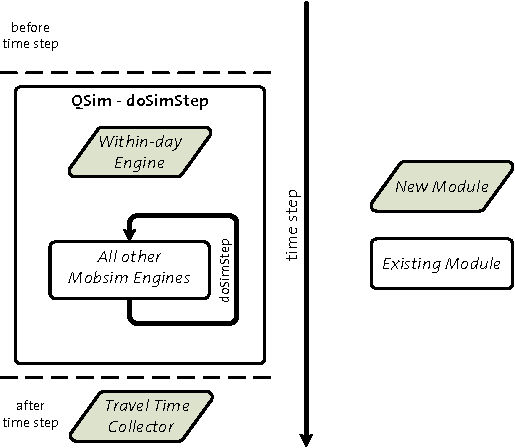
\includegraphics[width=8.0cm, angle=0]{extending/figures/WithinDayReplanning/QSimTimeStep}}%
{}
%---------------------------------------------------------------------

\mnote{example: TravelTimeCollector}

An example for such a class is the so-called \emph{TravelTimeCollector}. Its task is to provide actual link travel times to the \emph{Replanners} by collecting and averaging travel times of agents that have recently passed a link during a given time span. A typical time span is 15~minutes; older link travel times are ignored. Duration of the specific time span has an important impact on travel times reported to the \emph{Replanners}. On one hand, significant changes in link travel times will be communicated very slowly, if the time span is too long. On the other hand, a too short duration will overrate outliers.

The \emph{TravelTimeCollector} is a simple, but efficient implementation of a within-day travel time calculator. It does not implement features like traffic flow predictions or dynamic weighting of recent travel times based on historical data. 
%Due to 
Because of the abandonment of such features, it is very robust, even in scenarios where traffic flow conditions change dramatically.

%---------------------------------------------------------------------
\createfigure%
{TravelTimeCollector}%
{TravelTimeCollector}%
{\label{fig:labelTravelTimeCollector}}%
{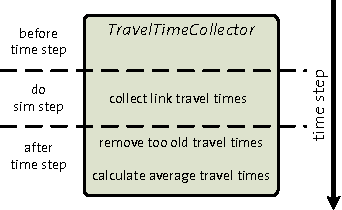
\includegraphics[width=8.0cm, angle=0]{extending/figures/WithinDayReplanning/TravelTimeCollector}}%
{}
%---------------------------------------------------------------------

\mnote{matsim person vs.\ matsim agent}

The current \acrshort{matsim} code differentiates between \lstinline$Person$ and \lstinline$MobsimAgent$.  
%
\lstinline$Person$ can be seen as a very simple Q-learning entity, possessing multiple \lstinline$Plan$s (``actions''), each together with an expected score which is updated every time the plan is tried out.  In consequence, a \lstinline$Person$ is persistent over the iterations; in fact, the internal state of each \lstinline$Person$ is written to file at the end of the iterations.
%
\lstinline$MobsimAgent$, in contrast, is instantiated every time the \lstinline$QSim$ is called, and does not exist beyond the running time of the \lstinline$QSim$.  A \lstinline$MobsimAgent$ is essentially reactive, being queried by the framework about decisions when approaching intersections, arrival points, or public transit stops.  In the standard implementation, these queries are answered by the plan, but other implementations can be used, and/or additional \lstinline$MobsimAgent$s can be added which do not correspond to \lstinline$Person$s.

\mnote{Which plan to modify}

This leads to the question if within-day adaptations to the \lstinline$Plan$ should be passed through to the \lstinline$Person$.  Let us call the actual trajectory through the system the ``executed plan''.  This can be different from the original plan, for example using a different route, different departure times, different modes, etc.  The original plan cannot just be replaced by the executed plan, since it is not clear that the executed plan, when used as input, will have itself as expected output.  In consequence, it is not possible to treat the executed plan together with the just obtained score as an action-value pair in the sense of Q-learning, since the score was obtained from the \emph{original} plan, not from the executed plan.

In consequence, the code uses a copy of the original plan and modifies the copy. The score, however, is given to the original plan. The implementation is able to 
\kai{``is able to''? (existiert das derzeit als Option?}
%
\dobi{Christoph: sollte da sein, sofern der Code nicht inzwischen zerschossen wurde. Ich hatte das für den Initial Routes Creation Abschnitt in meiner Diss verwendet. Ich wollte da auch nochmal genauer drauf schauen, was die produzierten Ergebnisse eigentlich bedeuten - habe ich dann aber irgendwie nie mehr Zeit dafür gefunden.}
% 
\emph{also} memorize the executed plan and add it to the set of plans. This functionality, however, is experimental.

%% \mnote{lskdjf}

%% An important aspect that has to be considered when within-day replanning is used is whether the persons' or only the agents' plans are replanned. In this context, a person is a global object which exists during an entire simulation run. An agent represents a person in the (traffic flow) micro-simulation part of an iteration. Moreover, a person has several plans in its memory, an agent only a single one. By default, an agent's plan is only a copy of the plan of the person which is represented. Only the score of the person's plan is updated by MATSim's scoring module. 

\mnote{parking example: parking search route should not be added to plan}

One example where setting the original to the executed plan clearly does not make sense is parking search \kai{citation?}
\dobi{Christoph: keine. Eventuell könntem an den Absatz auch weglassen? Der Standard ist ja mittlerweile, dass man den Plan der Person nicht verändert. Andererseits wäre dann der Absatz unten (mit den initial Routes) eher interessant, weil der eben ein Beispiel dafür gibt, wo die Standardeinstellung nicht sinnvoll ist.}.
\ah{\citet[][]{WaraichEtAl_TechRep_IVT_2013_2, WaraichEtAl_TechRep_IVT_2012}. Komme weder an den einen noch an den anderen dran und kann die Frage deshalb nicht selber beantworten.}
%In a first one, within-day replanning is used to simulate agents' parking search. 
A person's plan contains as destination the location where a free parking space is expected. However, if the agent realizes in the mobility simulation that there is no free space left, it starts looking for a free parking spot. As a result, the agent's route is extended. This extension has to be local in the agent's route since it is only necessary in the current iteration
but maybe not in another one where the initially selected parking spot is available.

%% \mnote{starting agents without routes: within-day routes \emph{should} be added to plan (but I don't agree)}

%Creating agents' initial routes using within-day replanning would be an example for an application where persons' plans have to be adapted. By default, creation of those routes is a step performed on person level before the micro-simulation is started for the first time. When this task is moved into the micro-simulation and is performed during their runtime, the created routes have to be still stored in the person's plan. Otherwise they would not be available for later iterations. 
%\kai{Christoph, habe hier mal tentativ einen Absatz auskommentiert, der mir nicht wirklich hilfreich erscheint.  Solange der Plan, mit dem der Agent losfährt, derjenige ist, der den Score bekommt, ist es unerheblich, wann er berechnet wurde.}
%\kai{some pointers to simulations done with this set-up}

The capabilities of this within-day replanning implementation are shown and discussed by \citet{Dobler_PhDThesis_2013} based on two sets of conducted experiments. The first set is based on a model of Zürich city. There it is assumed that the capacities of several arterial roads in the city center are drastically reduced during the morning peak. Traveling agents are given the opportunity to bypass the resulting traffic jams by adapting their routes using within-day replanning. As a result, the average travel time of an agent affected by the incident is reduced from 42 to 23 minutes. Another intersting finding is that even if only 50\% of the population adapts its routes still the average travel times are reduced to 25 minutes.
%\kai{Christoph: Vielleicht noch einen Satz über Ergebnisse (oder den vorhergehenden Satz umschreiben: Agents bypass the resulting traffic jams by adapting ..., leading to an overall readuction of travel times XX sec compared to the solution where agents stick to their routes.} 

The second set of experiments uses within-day replanning to create agents' initial routes. The results are compared to runs where those routes are created before the simulation is started and without having traffic flow information available. It is shown that agents' average travel times are already very close to the values in a relaxed state. When using MATSim's traditional approach, 10 to 15 iteration have to be performed before the average travel times have reached this level. %\kai{Christoph: Vielleicht noch einen Satz über Ergebnisse?}

\subsection{Implementation alternative~2: Replacing the agent}
\label{sec:impl-repl-the-ag}

According to \cite{RussellNorvigBook}, an agent is ``anything that can be viewed as perceiving its environment through sensors and acting upon that environment through effectors.''  As stated above, \acrshort{matsim} has agents on two levels:
\begin{compactitem}

\item \lstinline$Person$ is a Q-learning agent that is persistent over the iterations.

\item \lstinline$MobsimAgent$ is a reactive agent that only exists during the \lstinline$QSim$.

\end{compactitem}

For the Q-learning agent, perception works through the events, i.e.\ events are used to compute the score, build mental models to generate alternatives, etc.  Acting upon the environment works through the selection of the plan.

For the reactive agent, perception works more directly through callback methods, such as the simulation notifying the agent of just having moved over an intersection.  Acting upon the environment works through making decisions at decision points, e.g.\ about turning directions at intersections, or if to board a certain bus.

As said earlier, the approach described in Section~\ref{sec:impl-plan-based} assumes that the reactive agent still has, and most of the time follows, a plan.  There may, however, be situations where this is not appropriate, for example when the agent makes up the route as it goes, or when quite in general one wants to investigate models where each agent has its own perception and deliberation, rather than some external algorithm modifying its plan.  As also said earlier, there is no clear recipe when which approach is better; it depends both on the needs of the project and on the personal preferences of the developer.
%
Here, we will thus look at \lstinline$MobsimAgent$s which do no longer have a pre-compted plan but make decisions as they go.  There is also a class \lstinline$DynAgent$, which wraps around the somewhat archaic \lstinline$MobsimAgent$, making it easier to use and providing additional infrastructure (Section~\ref{sec:dynAgent}).

\subsubsection{Agent interface}

The \lstinline$DriverAgent$ interface structurally is something like
\begin{compactitem}

\item \lstinline$Id chooseNextLinkId()$ -- agent is asked at intersections and needs to return how to proceed.

%% \item \lstinline$Id<Link> getDestinationLinkId()$ -- agent is essentially asked if it wants to arrive on the current link.\footnote{%

%% The method can return {\tt null}.  Arguably, it should be modified to something like {\tt boolean isArrivingOnCurrentLink()}.

%% }  

\item \lstinline$boolean isWantingToArriveOnCurrentLink()$ -- agent is asked if it wants to arrive on the current link.

\item \lstinline$void notifyMoveOverNode(Id newLinkId)$ -- agent is notified that it has traversed the intersection and entered a new link.

\end{compactitem}
Everything else are relatively simple bookkeeping methods such as \lstinline$getId()$ -- the agent needs to know its own identifier.

If it is assumed that the agent does not only replan en-route but also while at activities, then also the \lstinline$MobsimAgent$ interface needs to be implemented.  This is a bit more involved; important methods are
\begin{compactitem}

\item \lstinline$endLegAndComputeNextState(...)$ -- agent is notified that the current transport leg has ended, and the agent internally needs to decide how to continue.

\item \lstinline$endActivityAndComputeNextState(...)$ -- agent is notified that the current activity has ended, and the agent internally needs to decide how to continue.

\item \lstinline$setStateToAbort(...)$ -- if a leg or an activity was not ended cleanly.  This can for example happen if \lstinline$chooseNextLinkId()$ returns a link that is not outgoing from the current node.\footnote{%
%
Despite the name of the method, the agent can recover.  %
}

\item \lstinline$getState()$ -- agent needs to return its current state, which essentially either returns \lstinline$ACTIVITY$ or \lstinline$LEG$.  The most important function of this is that the framework obtains the information if the agent wants to start a new activity or a new leg.

\end{compactitem}
Again, everything else are bookkeeping methods.

\subsubsection{Agent insertion}

The code accepts several ways to insert such a self-programmed \lstinline$MobsimAgent$ into the code, but the preferred way is using the \lstinline$AgentSource$ interface, as follows:
\begin{lstlisting}[basicstyle=\footnotesize\tt]{}
class MyAgentSource implements AgentSource {
   // constructor
   MyAgentSource ( Guidance guidance ) {
      ...
   }
   public void insertAgentsIntoMobsim() {
      // insert agent:
      MobsimAgent ag = new MyMobsimAgent( guidance ) ;
      qsim.insertAgentIntoMobsim(ag) ;
        
      // insert vehicle:
      Id<Vehicle> vehId = Id.create(ag.getId(), Vehicle.class);
      VehicleType vehType = VehicleUtils.getDefaultVehicleType();
      VehiclesFactory vehFactory = VehicleUtils.getFactory();
      Vehicle vehicle = vehFactory.createVehicle(vehId, vehType );
      Id<Link> linkId = null ; // replace by something meaningful
      qsim.createAndParkVehicleOnLink(veh, linkId );
   }
}
\end{lstlisting}
\lstinline$Guidance$ helps the agent with making decisions, see below.

\subsubsection{Perception, Decision, Integration}

The agents somehow need to perceive their environment.  The simulation tells the agent where it is, via \lstinline$notifyMoveOverNode(Id<Link> nextLinkId)$.  In general, however, this will not be enough.  For example, the agent may want to be informed about congestion, or evacuation directions.

A general way to achieve this is to use the \lstinline$Events$ channel.

We would probably suggest to separate observer, guidance, and the agent itself.

\paragraph{Observer}

The observer would probably listen to events:
\begin{lstlisting}
class MyObserver implements BasicEventHandler {
   @Override
   public void handleEvent(Event event) {
      ... // memorize information
   }
   ...
}
\end{lstlisting}

\paragraph{Guidance}

A guidance object might give guidance to the agents.  This could also be seen as a decision making entity.  This could, in principle, also be moved fully into the agent.  It could, for example, have the following design:
\begin{lstlisting}
class MyGuidance {
   MyGuidance( MyObserver observer ) {
      ...
   }
   Id<Link> chooseNextLinkId( Id<Link> currentLinkId ) {
      ... // compute and return decision
   }
}
\end{lstlisting}

\paragraph{Agent}

The agent would need access to the guidance:
\begin{lstlisting}
class MyAgent implements MobsimDriverAgent {
   MyGuidance guidance ;
   MyAgent( MyGuidance guidance ) {
      this.guidance = guidance ;
   }  
   ...
   @Override
   Id<Link> chooseNextLinkId() {
      return this.guidance.chooseNextLinkId( this.currentLinkId ) ;
   }
   ...
}
\end{lstlisting}

\paragraph{Control script}

This would be plugged together by a variant of the following script:
\begin{lstlisting}[basicstyle=\footnotesize\tt]{}
Controler ctrl = ... ;
...
// create observer object:
MyObserver observer = new MyObserver() ;
// add into events channel:
ctrl.addEventsHandler(observer) ;
// create guidance object:
MyGuidance guidance = new MyGuidance( observer ) ;
// create mobsim factory and set into controler:
ctrl.setMobsimFactory(new MobsimFactory(){
   public Mobsim createMobsim(Scenario sc, EventsManager ev ) {
      MobsimFactory factory = new QSimFactory() ; 
      QSim qsim = (QSim) factory.createMobsim(sc, ev) ;
      // add agent source into mobsim:
      qsim.addAgentSource( new MyAgentSource( guidance ) ) ;
      return qsim ;
   }
}) ;
...
ctrl.run() ;
\end{lstlisting}
The above ``script'' uses an anonymous class for the \lstinline$MobsimFactory$.  This way of writing code is quite convenient for adapting \acrshort{matsim} to one's need, also see Chap.~\ref{ch:extensionpoints}.

Code that compiles with the respective version of \acrshort{matsim} can be found in the package \lstinline$tutorial.programming.ownMobsimAgentWithPerception$ (e.g.\ to be found under \url{http://matsim.org/doxygen}).

\subsubsection{Using framework methods}

\acrshort{matsim} uses a wide range of methods to plan the day of a simulated traveler.  These can be passed into the guidance module, for example
\begin{lstlisting}
   Controler ctrl = new Controler(...) ;
   ...
   TripRouter router = ctrl.getTripRouterFactory().instantiateAndConfigureTripRouter() ;
   MyGuidance guidance = new MyGuidance( router ) ;
   ...
\end{lstlisting}
The guidance object can still be passed to the agent as before; it can now compute and then return, at each intersection, the best turn towards a destination.

Code that compiles with the respective version of \acrshort{matsim} can be found in the package \lstinline$tutorial.programming.ownMobsimAgentUsingRouter$ (e.g.\ to be found under \url{http://matsim.org/doxygen}).

\subsubsection{\lstinline{DynAgent}}

As stated earlier, there is also a class \lstinline$DynAgent$. It wraps around the somewhat archaic \lstinline$MobsimAgent$, making it easier to use and providing additional infrastructure (Section~\ref{sec:dynAgent}).
\mm{Kai, what do you mean by 'archaic'? In general, the architecture of DynAgent is much closer to the current version of PersonDriverAgentImpl.
DynAgentLogic produces next actions, like BasicPlanAgentImpl, and DynLegs (and DynActivities) are a kind of delegates for performing actions, like PlanBasedDriverAgentImpl is the delegate when it comes to driving.}

% ##################################################################################################################
% Local Variables:
% mode: latex
% mode: reftex
% mode: visual-line
% TeX-master: "../../main"
% comment-padding: 1
% fill-column: 9999
% End: 
